\section{Hauptteil} \label{sec:Hauptteil}
Der Hauptteil der Arbeit befasst sich mit der praktischen Umsetzung der Theorie. Der Code wird in Python implementiert und die verschiedenen Machine Learning Modelle werden auf die vorliegenden Daten angewendet. Die Modelle werden trainiert, getestet und die Ergebnisse werden ausgewertet und miteinander verglichen.

\subsection{Datenbeschaffung} \label{sec:Datenbeschaffung}
Die Daten wurden mithilfe eines Python-Skripts gesammelt, das täglich auf einem Raspberry Pi ausgeführt wird. Das Raspberry Pi sendet API-Anfragen an mehrere Datenanbieter und sammelt Informationen über die ausgewählte Aktie Adobe Inc., wie im ersten Teil beschrieben. Das Startdatum ist der 07.11.2023 und das Enddatum ist der 15.04.2024, um die Modelle vergleichbar zu machen. Die gesammelten Daten werden in einer CSV-Datei gespeichert. Insgesamt stehen 161 Datenpunkte zur Verfügung, auf denen die Modelle trainiert werden können.

\subsection{Datenanalyse} \label{sec:Datenanalyse}
Bevor die Daten verarbeitet werden, ist es sinnvoll, eine Analyse durchzuführen und die Struktur der Daten zu verstehen. Die Daten werden in ein Dataframe geladen und die ersten 5 Zeilen werden ausgegeben. Es wird überprüft, ob fehlende Werte vorhanden sind und die Datentypen der einzelnen Spalten werden überprüft. Die erste Zeile enthält das Datum des jeweiligen Tages, gefolgt von den Daten. Wenn die Daten von einem anderen Tag stammen, wird das Datum, an dem die Daten gesammelt wurden, angegeben. 
\par
Der Rohdatensatz enthält insgesamt 126 Spalten, darunter Daten in verschiedenen Formaten, Zahlen mit und ohne Nachkommastellen, Informationen über die Aktie und den CEO des Unternehmens und vieles mehr.
\begin{figure}[H]
    \centering
    \begin{tikzpicture}
        \node [anchor=south west] (image) at (0,0) {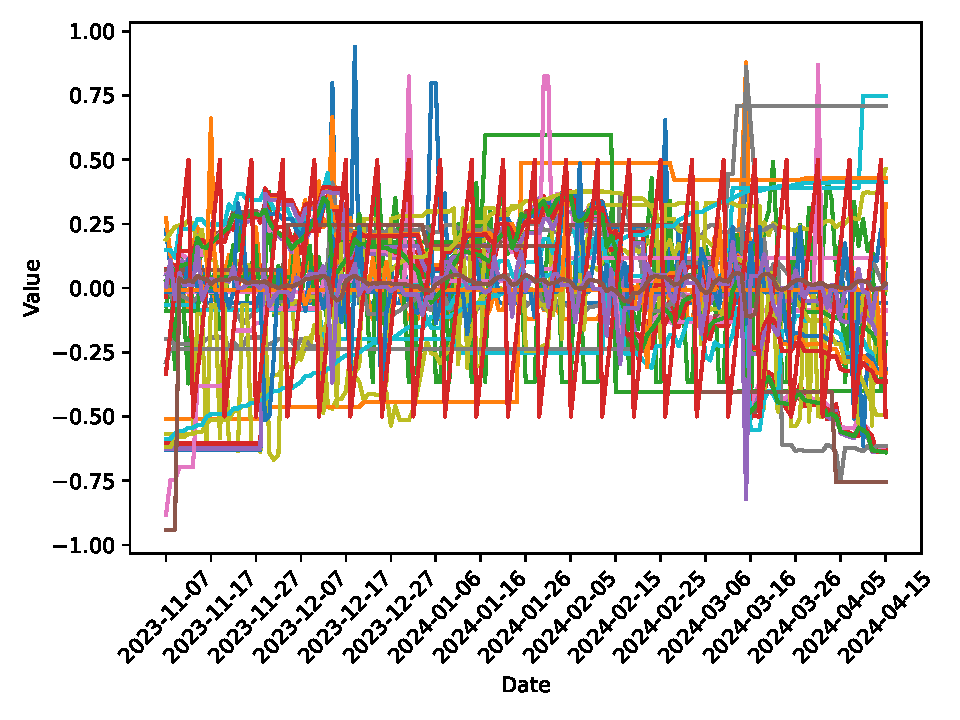
\includegraphics[width=1\textwidth,keepaspectratio]{Bilder/Features.pdf}};
    \end{tikzpicture}
    \caption{Features normalisiert}
    \label{fig: Features normalisiert}
\end{figure}
Die Features können nachdem sie normalisiert werden einzeln geplottet werden. \autoref{fig: Features normalisiert} zeigt alle Features in einem Plot, um die Verteilung der Daten zu visualisieren. Die einzelnen bunten Linien sind dabei die verschiedenen gesammelten Daten nach dem aussortieren von nicht-numerischen Daten. Die Daten sind normalisiert, um die Verteilung der Daten besser zu visualisieren. Die normalisierten Daten sind auf der y-Achse und die Anzahl der Datenpunkte (also die Tage) auf der x-Achse dargestellt.

\subsection{Rahmenprogramm}\label{sec:Rahmenprogramm}
Wie im Abschnitt \nameref{sec: Methodik} erläutert, wird ein \enquote{Rahmenprogramm} implementiert, das den gesamten Prozess strukturiert. Innerhalb dieses Rahmens können weitere Schritte zur Datenverarbeitung durchgeführt werden und die Modelle können wiederholt auf die Daten angewendet werden.

Der erste Schritt im Rahmenprogramm besteht darin, eine Funktion namens \enquote{logger} zu definieren. Die Logger Funktion funktioniert ähnlich wie das Print-Statement, speichert jedoch die Ausgabe in einer Datei. Der Logger wird in jedem Schritt des Programms verwendet, um die Ausgaben zu protokollieren. Dies ist wichtig, um die durchgeführten Schritte später nachvollziehen zu können, ohne das Programm erneut ausführen zu müssen. Der Aufruf des Loggers sieht wie folgt aus:

\begin{lstlisting}[language=Python, caption=Logger Initialisierung]
# Start des Programms, Zeitstempel wird protokolliert
logger("Das Programm wurde am " + str(datetime.now()) + " gestartet.")
\end{lstlisting}

Das Rahmenprogramm beginnt mit dem Einlesen der Rohdaten und der Konvertierung der ersten Spalte mit dem Datum in ein Datumsformat. Anschließend können die Daten sortiert werden. 

Es folgen Schritte, die erforderlich sind, um die Daten für die Anwendung der Machine Learning Modelle vorzubereiten. Das Rahmenprogramm soll sicherstellen, dass die Modelle trainiert werden können. Weitere Features können später hinzugefügt werden.

\begin{table}[H]
    \begin{tabularx}{\textwidth}{|c|X|}
        \hline
        \rowcolor{lightgray}
        \textbf{Schritt} & \textbf{Beschreibung} \\ \hline
        1 & Daten einlesen in einen Dataframe \\ \hline
        2 & Daten sortieren nach dem Datum\\ \hline
        3 & Platz für weitere Schritte, die in \autoref{tab:erklaerung_der_schritte} erklärt werden. \\ \hline
        4 & Alle nicht-numerischen Daten, wie Nachrichten entfernen\\ \hline
        5 & Leere Zellen füllen durch lineare Interpolation\\ \hline
        6 & Spalte erstellen, welche die Veränderung des Aktienwertes zum nächsten Tag in Prozent enthält (Target)\\ \hline
        7 & Daten in Trainings- und Testdaten aufteilen\\ \hline
        8 & Modelle trainieren und die Hyperparameter mit Randomized Search CV finden\\ \hline
        9 & Berechnung des Mean Squared Error und R2 Score für jedes Modell\\ \hline
        10 & Ergebnisse in einer Datei speichern \\ \hline
        11 & Ergebnisse analysieren und auswerten \\ \hline
        12 & Verschiedene Plots erstellen, um die Ergebnisse zu visualisieren.\\ \hline
    \end{tabularx}
    \caption{Schritte des Rahmens}
    \label{tab:schritte_des_rahmens}
\end{table}

Das Programm wird nach jeder Änderung, z.B. dem Hinzufügen eines Features, erneut ausgeführt und der Rahmen wird durchlaufen. Dadurch kann die Auswirkung der einzelnen Schritte, die an dritter Stelle eingefügt werden auf die Modelle genau betrachtet werden.

\subsection{Training der Modelle}\label{sec:Modelle}
Die verschiedenen Modelle haben unterschiedliche Hyperparameter, die gefunden werden müssen. Eine gängige Methode ist die Verwendung eines Gridsearch, bei dem alle möglichen Kombinationen von Hyperparametern ausprobiert werden. Dies ist jedoch rechenintensiv und zeitaufwändig.
\par
Ein alternativer Ansatz ist die Verwendung des RandomizedSearchCV, wie in \autoref{sec: Randomized Grid Search} erläutert. Da das Programm auf einem handelsüblichen Laptop ausgeführt wird, wird diese Methode gewählt, da sie weniger rechenintensiv ist.
\par
Die Modelle werden in einer Schleife trainiert und getestet und in einer Liste mit ihren Hyperparametern gespeichert. Die Ergebnisse werden in einer Datei gespeichert und können später ausgewertet werden.

Ein Teil der Liste sieht wie folgt aus:

\begin{lstlisting}[language=Python, caption=Liste der Modelle]
    models = [
        {
            "name": "Lineare Regression",
            "model": LinearRegression(),
            "param_grid": {}
        },
        {
            "name": "KNN",
            "model": KNeighborsRegressor(),
            "param_grid": {
                'n_neighbors': [3, 5, 11, 19],
                'weights': ['uniform', 'distance'],
                'metric': ['euclidean', 'manhattan']
            }
        }
    ]
\end{lstlisting}

Der Listenauschnitt enthält die Lineare Regression und den KNN Regressor. Der KNN Regressor hat Hyperparameter, die getestet werden müssen, während die Lineare Regression keine Hyperparameter hat.

Der RandomizedSearchCV kann dann einfach wie folgt aufgerufen werden, um die besten Hyperparameter für das Modell zu finden:

\begin{lstlisting}[language=Python, caption=RandomizedSearchCV]
    random_search = RandomizedSearchCV(model["model"], model["param_grid"], n_iter=5, cv=5, n_jobs=-1, verbose=2)
    random_search.fit(X_train, y_train)
\end{lstlisting}

Der RandomizedSearchCV wird für jedes Modell in der Liste aufgerufen, indem eine Schleife über die Liste läuft.

\subsection{Datenverarbeitungsschritte}\label{sec:Datenverarbeitungsschritte}
Die Datenverarbeitungsschritte sind die Schritte, die nachträglich in den Rahmen eingefügt werden. Nach jedem der unten aufgelisteten Schritte werden die Modelle erneut trainiert und getestet.

Die Tabelle zeigt die Datenverarbeitungsschritte als Index und den Wert des jeweiligen Modells. Der Wert in der Tabelle ist der Gesamtscore, der im Abschnitt \nameref{sec: Benchmarks} eingeführt wurde.

\begin{table}[H]
    \centering
    \begin{tikzpicture}
        \node [anchor=south west] (image) at (0,0) {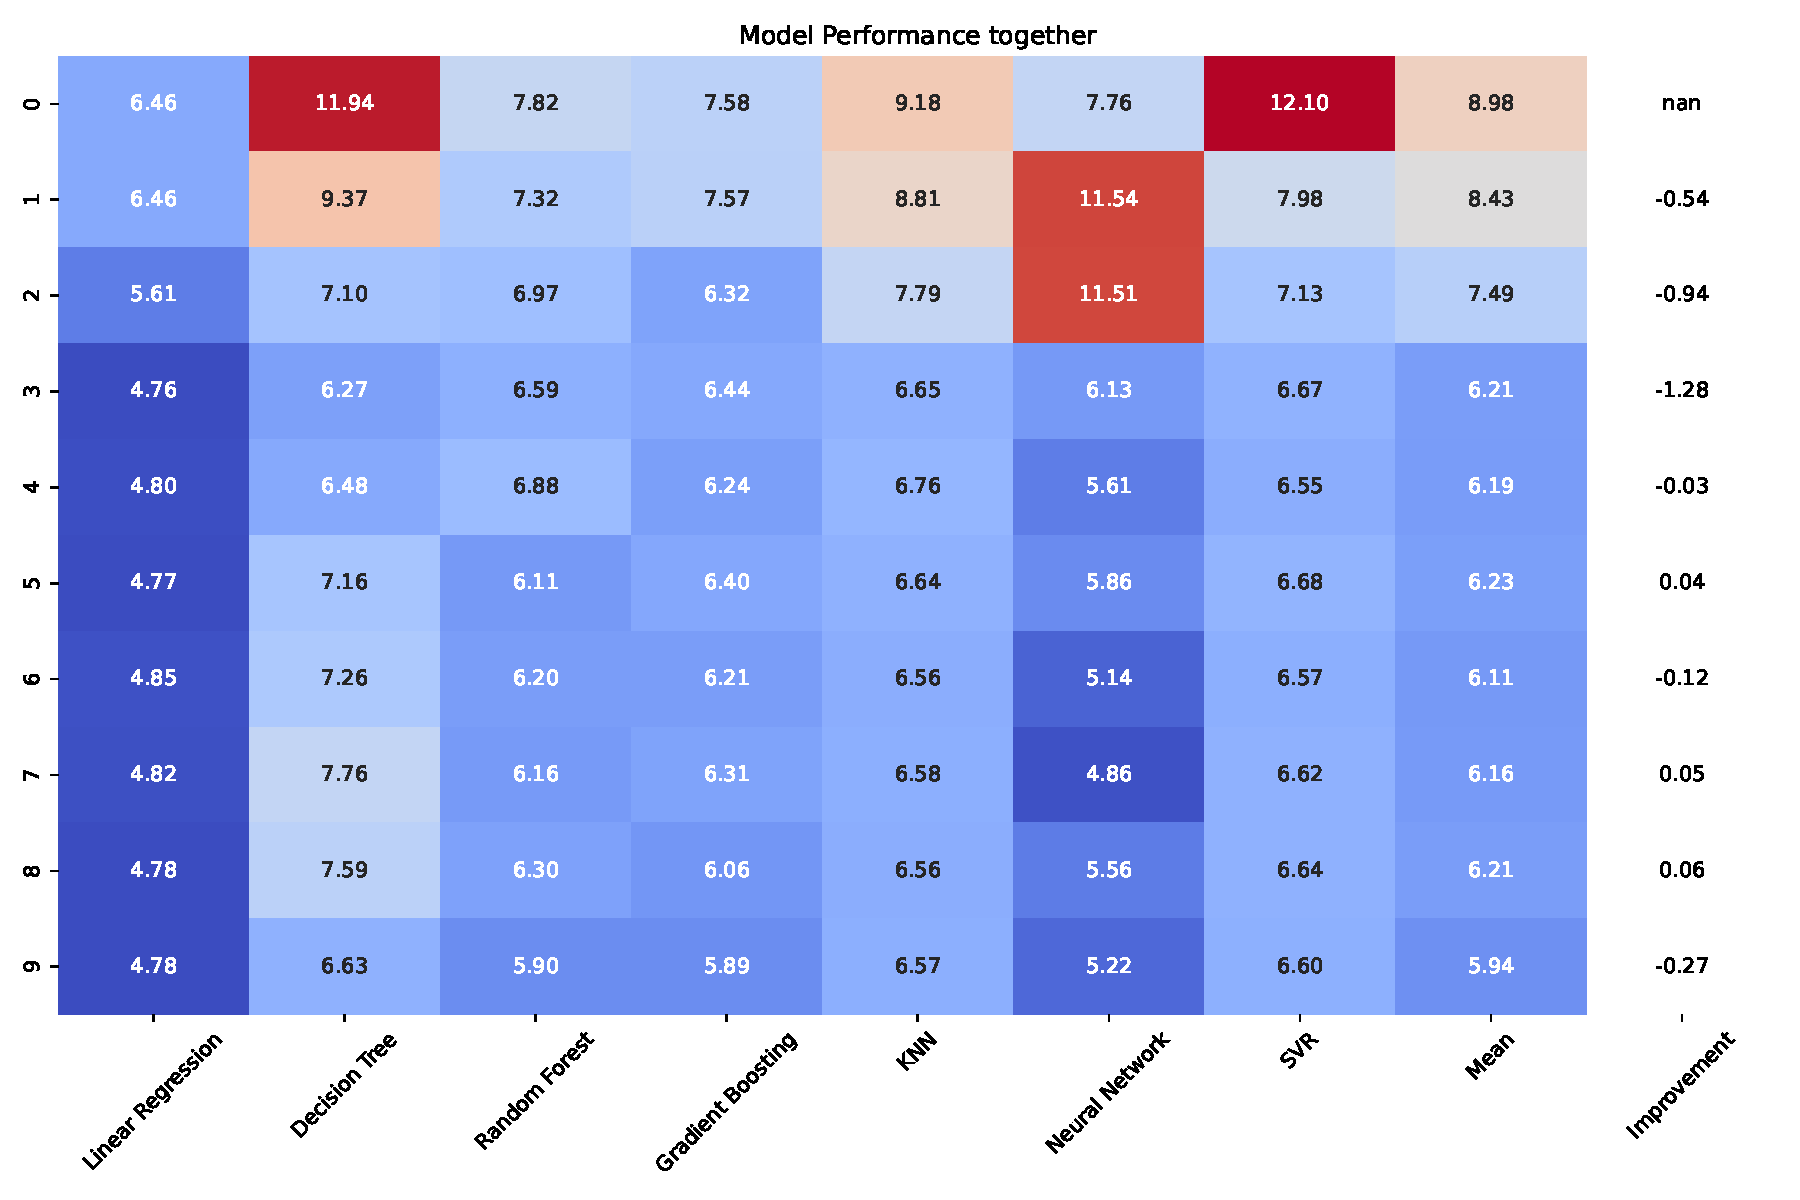
\includegraphics[angle = 90,width=1\textwidth,keepaspectratio]{Bilder/colored_table_together.pdf}};
    \end{tikzpicture}
    \caption{Gesamtscore}
    \label{tab:Gesamtscore}
\end{table}

\begin{table}[H]
    \begin{tabularx}{\textwidth}{|c|X|}
        \hline
        \rowcolor{lightgray}
        \textbf{Schritt} & \textbf{Beschreibung} \\ \hline
        0 & \textbf{Entfernung nicht-numerischer oder spärlicher Merkmale}: Nicht-numerische Merkmale sowie Merkmale mit weniger als fünf Werten wurden aus dem Datensatz entfernt, um die Qualität der Analyse zu verbessern. \\ \hline
        1 & \textbf{Datenstandardisierung mit Z-Score}: Die Daten wurden mittels Z-Score standardisiert, um die Mittelwerte auf 0 und die Standardabweichungen auf 1 zu normieren. \\ \hline
        2 & \textbf{Lineare Interpolation für Wochenendwerte}: Für fehlende Werte an Wochenenden wurde eine lineare Interpolation durchgeführt, um eine kontinuierliche Datensequenz zu gewährleisten. \\ \hline
        3 & \textbf{Berechnung des nächsten Tagespreises mit Durchschnittspreis}: Anstelle des Schlusspreises wurde der Durchschnittspreis verwendet, um die prozentuale Preisänderung des folgenden Tages zu berechnen. \\ \hline
        4 & \textbf{Wochentagkodierung von 0 bis 6}: Die Wochentage wurden als ganze Zahlen von 0 (Montag) bis 6 (Sonntag) kodiert, um eine eindeutige und effiziente Verarbeitung zu ermöglichen. \\ \hline
        5 & \textbf{Preisänderung im Vergleich zum Vortag}: Die Preisänderung im Vergleich zum Vortag wurde berechnet, um kurzfristige Markttrends analysieren zu können. \\ \hline
        6 & \textbf{Preisänderung im Vergleich zu drei Tagen zuvor}: Die Preisänderung im Vergleich zu drei Tagen zuvor wurde ermittelt, um mittelfristige Preisbewegungen zu erfassen. \\ \hline
        7 & \textbf{Sentimentanalyse mit Finbet}: Tägliche Sentiment-Scores wurden unter Verwendung von Finbet generiert, indem CEO- und Unternehmensnachrichten analysiert und in Stimmungswerte übersetzt wurden. \\ \hline
        8 & \textbf{Verwendung des Standard Scalers}: Anstelle des Z-Scores wurde der Standard Scaler aus sklearn für die Datenstandardisierung verwendet, um eine Alternative zur Z-Score-Methode zu bieten. \\ \hline
        9 & \textbf{PCA mit automatischer Dimensionsreduktion}: Die Hauptkomponentenanalyse (PCA) wurde angewandt, wobei die Anzahl der Komponenten automatisch basierend auf der erklärten Varianz ausgewählt wurde. \\ \hline
    \end{tabularx}
    \caption{Erklärung der Schritte}
    \label{tab:erklaerung_der_schritte}
\end{table}
Das beste Modell wird ausgewählt und verwendet, um die Preisänderung für den nächsten Tag vorherzusagen. Der folgende Graph zeigt die tatsächliche und die vorhergesagte Preisänderung.

\begin{figure}[H]
    \centering
    \begin{tikzpicture}
        \node [anchor=south west] (image) at (0,0) {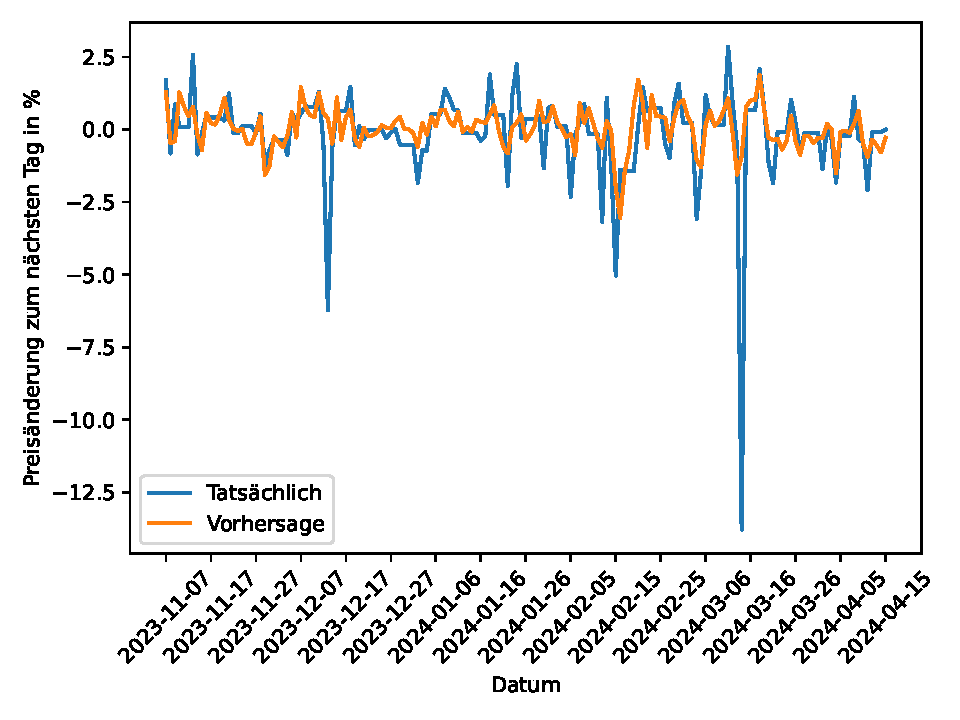
\includegraphics[width=1\textwidth,keepaspectratio]{Bilder/Predictions.pdf}};
    \end{tikzpicture}
    \caption{Vorhersage der Preisänderung}
    \label{fig:Predictions}
\end{figure}

\subsection{Anwendung}\label{sec:Anwendung}
Die Modelle sagen die Preisänderung für den nächsten Tag voraus. Da die Nachrichten und Daten von den API-Providern in der kostenfreien Version nur mit einem Tag verzögerung verfügbar sind, muss bei der Anwendung auf die Uhrzeit geachtet werden. Die Berechnung und Vorhersage erfolgen morgens vor der Öffnung des Marktes um 07:00 Uhr.
\par
Um eine Vorhersage zu treffen, wird das Modell mit dem besten Gesamtscore ausgewählt und auf alle verfügbaren Daten angewendet.
\par
Es ist jedoch wichtig zu beachten, dass die Vorhersage eine Preisänderung in Prozent ist und kein Kauf- oder Verkaufssignal. Wie aus der prozentualen Preisänderung ein Handelssignal abgeleitet wird, wird im Abschnitt \nameref{sec: VorhergesagteProzentezuHandelssignale} erläutert.

\subsection{Vorhergesagte Prozente zu Handelssignalen}\label{sec: VorhergesagteProzentezuHandelssignale}
Die Vorhersage gibt die prozentuale Preisänderung an. Diese Änderung kann positiv oder negativ sein. Um aus der Preisänderung ein Handelssignal abzuleiten, wird ein Schwellenwert festgelegt. Wenn die Änderung größer als der Schwellenwert ist, wird ein Kaufsignal generiert. Wenn die Änderung kleiner als der Schwellenwert ist, wird ein Verkaufssignal generiert.
\par
Dieser Schwellenwert muss optimiert werden. Hierfür wird das zuvor beschriebene \nameref{sec: Optuna} verwendet. Optuna sucht den besten Schwellenwert innerhalb eines festgelegten Bereichs. Für ein Verkaufssignal wird ein Bereich von 0 \% bis -10 \% und für ein Kaufsignal ein Bereich von 0 \% bis 10 \% gewählt. Optuna benötigt jedoch eine Funktion, die optimiert werden kann. Hierfür wurde ein Simulationsprogramm entwickelt. Optuna versucht, den Depotwert zu maximieren, der sich aus dem Kauf und Verkauf der Aktie ergibt. Der Ablauf ist wie folgt:

\begin{enumerate}
    \item Es gibt zwei Konten: das Depot und das Cash. Anfangs befinden sich 500 € im Depot und 500 € in Cash.
    \item Optuna wählt zwei Schwellenwerte, einen für den Kauf und einen für den Verkauf.
    \item Wenn die vorhergesagte Änderung größer als der Kaufschwellenwert ist, wird so viel von der Aktie gekauft, bis das Cash aufgebraucht ist. Ein Kauf kostet außerdem 1 € Gebühr.
    \item Wenn die vorhergesagte Änderung kleiner als der Verkaufschwellenwert ist, wird 50 \% des Depots verkauft. Ein Verkauf kostet ebenfalls 1 € Gebühr. Das Depot wird dann in Cash umgewandelt.
\end{enumerate}

Optuna führt diesen Ablauf für eine festgelegte Anzahl von Iterationen durch und versucht, den Depotwert zu maximieren. Der Depotwert ist die Summe aus Cash und Depotwert.

Am Ende erhält man die besten Schwellenwerte für den Kauf und den Verkauf. Diese Schwellenwerte werden dann in der Anwendung verwendet, um aus der Vorhersage ein Handelssignal abzuleiten.\autoref{fig: Optuna Parallel Plot} zeigt die Ergebnisse von Optuna. In der Mitte ist der Buy Threshold und auf der rechten Seite der Sell Threshold. Links im Graph ist der Depotwert dargestellt, den es zu maximieren gilt. Die Linien zeigen die verbindungen zwischen den einzelnen Punkten, also bei welchen Parametern, welcher Depotwert erreicht wurde.
\begin{figure}[H]
    \centering
    \begin{tikzpicture}
        \node [anchor=south west] (image) at (0,0) {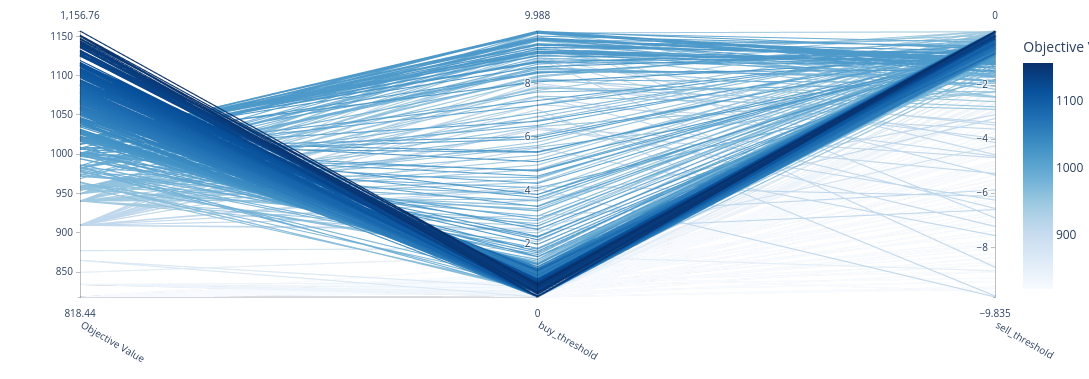
\includegraphics[width=1\textwidth,keepaspectratio]{Bilder/optuna_parallel_plot.png}};
    \end{tikzpicture}
    \caption{Optuna Parallel Plot}
    \label{fig: Optuna Parallel Plot}
\end{figure}
Des Weiteren lässt sich der Verlauf der Optimierung in einem Graphen darstellen. \autoref{fig: Optuna Verlauf} zeigt den Verlauf der Optimierung. Links ist wieder der Depotwert dargestellt, der maximiert werden soll. Die horizontale Achse zeigt die Anzahl der Iterationen. Die Punkte sind die Versuche und die rote Linie zeigt den Verlauf der besten Werte. Die besten Werte sind die, die den Depotwert maximieren.
\begin{figure}[H]
    \centering
    \begin{tikzpicture}
        \node [anchor=south west] (image) at (0,0) {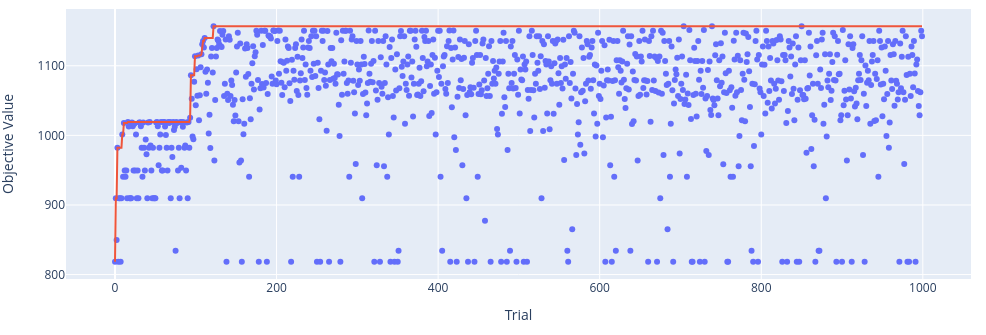
\includegraphics[width=1\textwidth,keepaspectratio]{Bilder/optuna_optimization_history.png}};
    \end{tikzpicture}
    \caption{Optuna Verlauf}
    \label{fig: Optuna Verlauf}
\end{figure}

\subsection{Ergebnisse}\label{sec:Ergebnisse}
Die Ergebnisse sind zur übersichtlichen Darstellung in einer Tabelle zusammengefasst.

\begin{table}[H]
    \begin{tabularx}{\textwidth}{|l|X|}
        \hline
        \rowcolor{lightgray}
        \textbf{Beschreibung} & \textbf{Ergebniss} \\ \hline
        Bestes Modell & Lineare Regression\\ \hline
        Gesamtscore (siehe \autoref{sec: Benchmarks}) & 4.78\\ \hline
        Schwellenwert Kauf & 0,46 \%\\ \hline
        Schwellenwert Verkauf & -0,011 \%\\ \hline
        Erreichter Depotwert & 1156,76 €\\ \hline
        Erreichte Differenz zur Haltstrategie & 33,93 \%\\ \hline
    \end{tabularx}
    \caption{Schritte des Rahmens}
    \label{tab:schritte_des_rahmens}
\end{table}

Mit den vorhergesagten Werten und den Schwellenwerten gibt es für jeden Tag ein Kauf-, Halt- oder Verkaufssignal. Diese Signale werden in einem Graphen dargestellt, wobei grüne oder rote Balken verwendet werden.

Bei einem Kauf wird das Cash in die Aktie investiert, bei einem Verkauf wird 50 \% des Depots verkauft. 

Der folgende Graph zeigt den Verlauf der Simulation, bei der die Signale berücksichtigt werden und der Aktienwert normalisiert wird, um eine vergleichbare Skalierung zu gewährleisten.

\begin{figure}[H]
    \centering
    \begin{tikzpicture}
        \node [anchor=south west] (image) at (0,0) {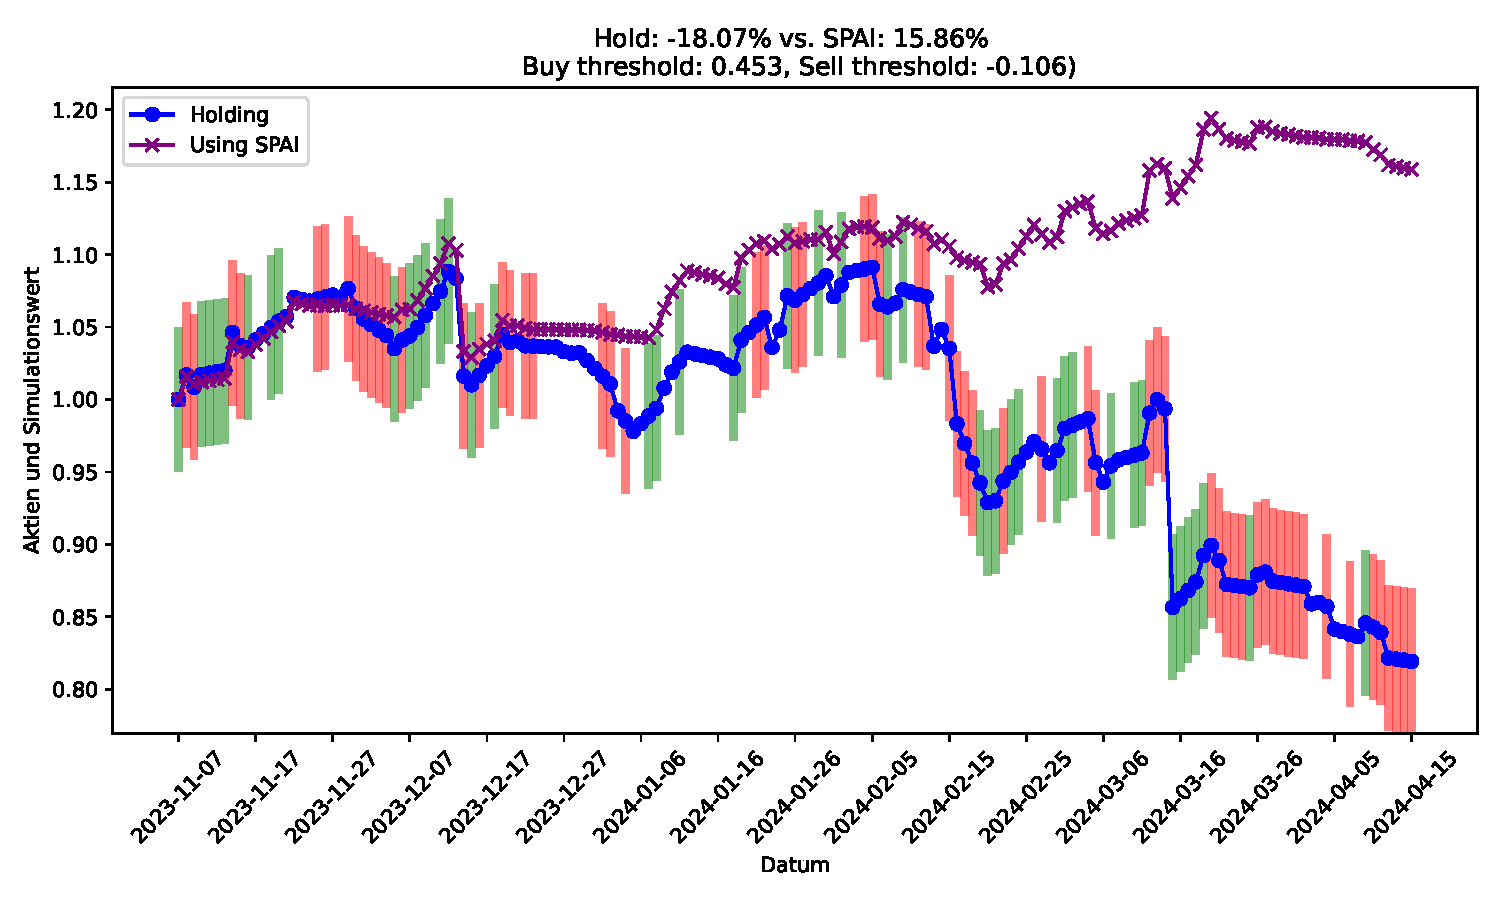
\includegraphics[angle = 90,height=0.9\textheight,keepaspectratio]{Bilder/Simulation.pdf}};
    \end{tikzpicture}
    \caption{Simulation mit Handelssignalen}
    \label{fig:Simulation}
\end{figure}